\documentclass[11pt]{article}
\usepackage{colacl}
\usepackage{graphicx}
\usepackage[T1]{fontenc}
\usepackage[utf8]{inputenc}
\usepackage{amsmath}
\usepackage{bm}
\graphicspath{{img/}}
\DeclareUnicodeCharacter{F8FF}{$\diamond$}
\sloppy

\title{COMP30027 Assignment 2: Report}
\author
{Anonymous}



\begin{document}
\maketitle

\section{Introduction}\label{sec:intro}
% Introduction: a short description of the problem and data set

Sentiment analysis is a field of natural language processing focusing on the classification of text by its perceived sentiment.
It speeds up measuring the opinions of groups of people and can be applied in many fields such as marketing, politics or sociology.
My goal is to develop and train three differenct reliable {T}witter sentiment classifiers and one baseline model.
This involves developing methods to extract and select useful features from a dataset of posts, 
then to choose and evaluate highly reliable classifier models.

\subsection{Dataset}\label{sec:dataset}

The given dataset provided contains two lists of {T}witter posts (tweets) made on the platform prior to 2017 \cite{dataset}.
The two files enclosed are a \texttt{Train.csv} for training and a \texttt{Test.csv} for testing. 
Each tweet is an instance in the dataset.
The training set contains $21802$ labelled instances and the testing set contains $6099$ instances. 
For each instance, included is the tweet text and tweet ID. 
The tweets included vary in content.
For example, some tweets are not entirely in English: ``\textit{season in the sun versi nirvana rancak gak..slow rockkk...}''.
In the training file also contains the true sentiment of each tweet. 
Tweets can either have a "positive", "neutral" or "negative" sentiment, distributed as shown in Figure~\ref{fig:sent-dist}.

\begin{figure}[!h]
	\centering
	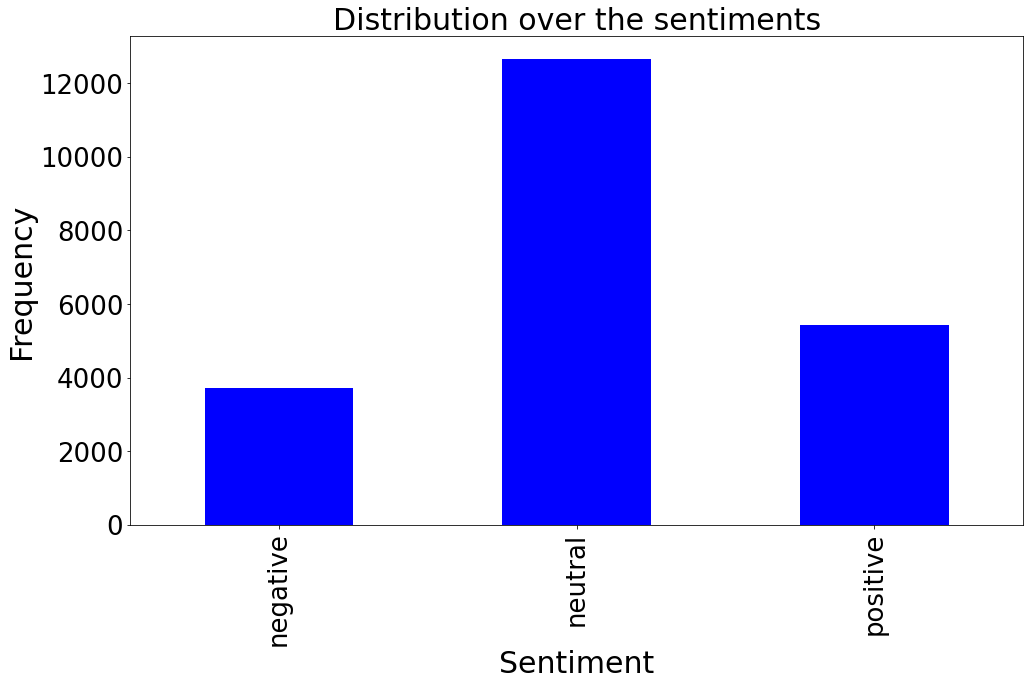
\includegraphics[width = 0.42\textwidth]{sentiment-distribution.png}
	\caption{Distribution of the sentiments}
	\label{fig:sent-dist}
\end{figure} 

\section{Methodology}
% Method: Introduce the used feature(s), and the rationale behind including them. Explain the classifiers
% and evaluation method(s) and metric(s) you have used (and why you have used them). This should be
% at a conceptual level; a detailed description of the code is not appropriate for the report. The description
% should be similar to what you would see in a machine learning conference paper.

This section contains a breakdown of the process through which the final models are developed.
The following methods are developed with reference to prior works on {T}witter sentiment analysis by Go et al. \shortcite{go09} and Barbosa and Feng \shortcite{robustnoisy10}.

\subsection{Instance cleaning}

Some of the features extracted rely on the text in the tweets to be pruned of unwanted characters and words.
I have opted to generate a separate list containing the cleaned versions of tweets.
Cleaning involves removing stopwords (Section~\ref{sec:stopwords}), links, tweet hashtags, tweet mentions, numbers, non-alphanumeric characters.
Also performed is the reduction of repeated letters with more than two occurrences to just two, as suggested by Go et al. \shortcite{go09}.

Neither stemming nor lemmatization are used in the final models as I consider both too language-dependent
to be useful in non-English instances.

\subsubsection{Stopwords}\label{sec:stopwords}

Manual stopword list construction is tedious and inexhaustive (I cannot identify stopwords in certain languages). 
Therefore, I have opted to start with the {P}ython Natural Language Toolkit's (\texttt{NLTK}) defined stopword list, which includes multiple languages \cite{nltk}.
To test the efficacy of this set, 
I generate a set of word clouds over the training cleaned tweets (using the \texttt{NLTK} stopword list) grouped by sentiment.
This then informs whether more terms need to be manually added the used list does not include.

\subsection{Feature extraction}

\subsubsection{How many features per feature type is enough?}

With over 20000 instances in the training dataset, some of the feature types defined will generate a massive range of results.
When vectorizing, it is best practice to implement a hard maximum for the unique number of features in a feature type.
To determine this number $M_f$, the top candidate classifiers are compared for each of $M_f \in \lbrace 10, 100, 1000, 5000 \rbrace$ by the accuracies found using Section~\ref{sec:choosing2}.

\subsubsection{{T}witter features}

First, relying on personal usage experience with {T}witter, I extract the main platform-specific features from the tweet text.
These are:
\begin{itemize}
	\item Hashtags (e.g. \texttt{\#term}): Used to associate tweets with a certain term on the platform.
	\item Mentions (e.g. \texttt{@user}): Used when addressing a specific user on the platform.
	\item Links (e.g. \texttt{https://t.co/id}): Used to link to a website with an id on the platform's redirect service.
\end{itemize}  

These are integrated within the {T}witter platform, meaning they are widely used by users.
Therefore, these features may be strongly correlated to the sentiments and should be isolated for use in the final models.

\subsubsection{Linguistic features}

Next, linguistic features are extracted and used to tokenize the tweet in different ways. 

\begin{itemize}
	\item Part-of-Speech Tags: Extracting the grammatical types of words.
	\item Words
	\item Word 2-Grams: Word pairs used in the tweet.
	\item Word Lengths: The lengths of words used as tokens.
	\item Phonetics: The phenomes of english words as defined in the CMU Pronounciation Dictionary \cite{cmudict}.
	\item Alphabetic Characters
	\item Punctuation (\texttt{.?!,:;-()[]\{\}"'/})
\end{itemize}  

These feature types may all have features which are strongly correlated to sentiments.
For example, a positive \texttt{big win} versus a negative \texttt{big disaster} word 2-gram.

\begin{itemize}
	\item Emoticons (e.g. \texttt{:(} or \texttt{:)}): The rise of \texttt{ASCII} emoticons allows users to quickly express their emotions, which correlate strongly to the sentiment of their text.
\end{itemize}  

Extracting emoticons is done differently to the method used in the Go et al. \shortcite{go09} research,
since their method misses a large number of emoticons, such as the surprised duck \texttt{:v} emoticon.
Instead, emoticons are defined as a string comprised of eyes (\texttt{;:8=}), optional middle characters (\texttt{,'-"*}), 
and mouths divided into categories: happy (\texttt{)3]}), sad (\texttt{\\/([}), neutral (\texttt{pl|}) and surprised (\texttt{vo}).
The detected emoticons (including reversed versions) are simplified into one of four emoticons based on their mouth category: happy \texttt{:)}, sad \texttt{:(}, neutral \texttt{:|} and surprised \texttt{:o}.

\subsubsection{Metric features}

These are largely numeric counts of the previously mentioned feature types within a tweet.

\begin{itemize}
	\item Number of Words
	\item Number of Characters
	\item Number of Alphabetic Characters
	\item Number of Links
	\item Number of Hashtags
	\item Number of Mentions
	\item Number of Emoticons
	\item Quoting (e.g. \texttt {"text"}): Can also be called \emph{retweets}, represented in the dataset with quote marks.
	\item Average Word Length
\end{itemize}

These metrics can help differentiate between a neutral tweet and a sentimental tweet (e.g. emoticons are correlated to emotion).

% \begin{itemize}
% 	\item \textbf{Poetic Phonetics}: The counts of occurrences of sibilance, fricatives and plosives, detected using the phenomes of words \cite{tsur2019phonetic,cmudict}.
% \end{itemize}

% The significance of phonetic symbolism is highly debated, however, out of personal curiosity, I have decided to included this set.

\subsubsection{Vectorization}

For all non-metric feature types, they can be vectorized by $TF$-$IDF$, or by occurrence counts.
At the time that the data was collected, tweets were limited to 140 characters \cite{tweetlen}.
This suggests that most features (including word pairs) will only appear at most once in a tweet.
Therefore, non-metric features are vectorized with their occurrence counts. 

% \subsubsection{Bar graph comparison test}\label{sec:bargraphs}

% One way I use to determine the predictive potential of a feature is through comparitive bar graphs.
% I generate bar graphs comparing the distributions over the top 10 features in a feature set by the proportion of their values, such that:
% \begin{equation*}
% 	\emph{proportion}_{\bm{\sigma} \subseteq S} = \frac{\sum f_{\bm{\sigma} \subseteq S}}{\sum f_S}
% \end{equation*}
% where $\bm{\sigma}$ is a subset of all the sentiments $S$, $f$ is the vector of values per tweet for a specific feature in a feature type.
% If too many of the same features appear in all sentiments' bar graphs, then the feature type is considered weaker for the model fit.

\subsection{Classifier Selection}

\subsubsection{Baseline}

The baseline model used will be 0-R: most frequent class.
All chosen models need to outperform this one.

\subsubsection{Classifiers Considered}

The following classifiers and parameters are first all measured as described in Section~\ref{sec:choosing2}:

\textbf{Multinomial/Bernoulli Naive Bayes}:
Naive bayes classifiers each assuming likelihood distributions of features corresponding to their name.
\begin{table}[h]
	\begin{center}
		\begin{tabular}{|c|c|}			
			\hline
			Parameter & Values Considered \\
			\hline\hline
			Include Label Priors & Yes, No \\
			Alpha Smoothing ($\alpha$) & 0, 1, 10 \\
			\hline
		\end{tabular}
		\caption{Naive Bayes Parameter Sets}
		\label{tbl:nb-options}
	\end{center}
\end{table}

\textbf{Logistic Regressions}:
Linear statistical models for categorical labels. 
\begin{table}[h]
	\begin{center}
		\begin{tabular}{|c|c|}			
			\hline
			Parameter & Values Considered \\
			\hline\hline
			Fit Intercept & Yes, No \\
			Maximum Iterations & 100, 500 \\
			Optimizer Algorithm & \texttt{sag}, \texttt{saga} \\
			\hline
		\end{tabular}
		\caption{Logistic Regression Parameter Sets}
		\label{tbl:lr-options}
	\end{center}
\end{table}

\textbf{Decision Trees}:
Branching tree classifiers. 
\begin{table}[h]
	\begin{center}
		\begin{tabular}{|c|c|}			
			\hline
			Parameter & Values Considered \\
			\hline\hline
			Maximum Depth & 1, 100, 500 \\
			\hline
		\end{tabular}
		\caption{Decision Tree Parameter Sets}
		\label{tbl:dt-options}
	\end{center}
\end{table}

\textbf{$K$ Nearest Neighbours}:
Decides classes based on the $K$ closest neighbours' class labels (in a weighted voting system). 
\begin{table}[!h]
	\begin{center}
		\begin{tabular}{|c|c|}			
			\hline
			Parameter & Values Considered \\
			\hline\hline
			$K$ Neighbours & 1, 10, 100, 500 \\
			Vote Weighting & \texttt{uniform}, \texttt{distance} \\
			\hline
		\end{tabular}
		\caption{K-Nearest Neighbour Parameter Sets}
		\label{tbl:knn-options}
	\end{center}
\end{table}

\textbf{Support Vector Classifiers}:
Create borders between classes with the use of support vectors. 
\begin{table}[!h]
	\begin{center}
		\begin{tabular}{|c|c|}			
			\hline
			Parameter & Values Considered \\
			\hline\hline
			Kernel Function & Linear, Cubic \\
			Regularization $C$ & 0.1, 1, 3 \\
			Decision Function & One-v-One, One-v-Rest \\
			\hline
		\end{tabular}
		\caption{Support Vector Classifier Parameter Sets}
		\label{tbl:svc-options}
	\end{center}
\end{table}


\subsection{Evaluation}\label{sec:evaluations}

\subsubsection{Which Classifier/Parameter Configurations Are Best?}\label{sec:choosing2}

To reduce the inital set of possible estimators to just two selected candidates,
they are each cross-validated twice. 
First, 5-fold cross validation scores are calculated on the dataset as is.
Then, 5-fold cross validation scores are calculated on largest subset of the data with a uniform distribution of sentiments.
These 10 scores are then averaged $\bar{x}$, and their standard deviations $s$ found. 
The top candidate classifier/parameter configurations are found based on the highest approximate $80\%$ lower bounds ($\bar{x} - s$).


\subsubsection{Evaluation Metrics}\label{sec:evalmetrics}

The following metrics are generated for each classifier that makes it past Section~\ref{sec:choosing2}:
\begin{table}[!h]
	\begin{center}
		\begin{tabular}{|c|c|}			
			\hline
			Metric & Formula \\
			\hline\hline & \\
			Accuracy & $\frac{\#\emph{Correct}}{n}$ \\ & \\
			Precision (per class) & $\frac{TP}{TP + FP}$ \\ & \\
			Recall (per class) & $\frac{TP}{TP + FN}$ \\ & \\
			$F_1$-Score (per class) & $\frac{2TP}{2TP + FP + FN}$ \\ & \\
			\hline
		\end{tabular}
		\caption{Metrics calculated for chosen models}
		\label{tbl:cand-metrics}
	\end{center}
\end{table}

On top of this, the model's confusion matrix is also generated, for visual representations potential biases.

\subsubsection{Which models are label distribution agnostic?}

It is unknown whether the \texttt{Text.csv} labels are distributed similarly to those in \texttt{Train.csv}.
Therefore evaluation metrics are generated on four $4:1$ train to test sets.
First are generated a set of training and testing sets on the maximum subset of the data with uniform sentiment distribution.
Next are generated a set of training and testing sets on the data with sentiments distributed as given (Randomly).
From these, four sets of evaluation metrics are generated:
\begin{itemize}
	\item Uniform Training and Random Testing
	\item Uniform Training and Uniform Testing
	\item Random Training and Random Testing
	\item Random Training and Uniform Testing
\end{itemize}

The evaluation metrics as generated in Section~\ref{sec:evalmetrics} are then compared to see which of the models 
(including the baseline) are most agnostic to sentiment distributions.

\section{Results}\label{sec:results}
% Results: Present the results, in terms of evaluation metric(s) and, ideally, illustrative examples and diagrams.

\subsection{Comparing the effects of stopword removal}

\begin{figure}[!h]
	\centering
	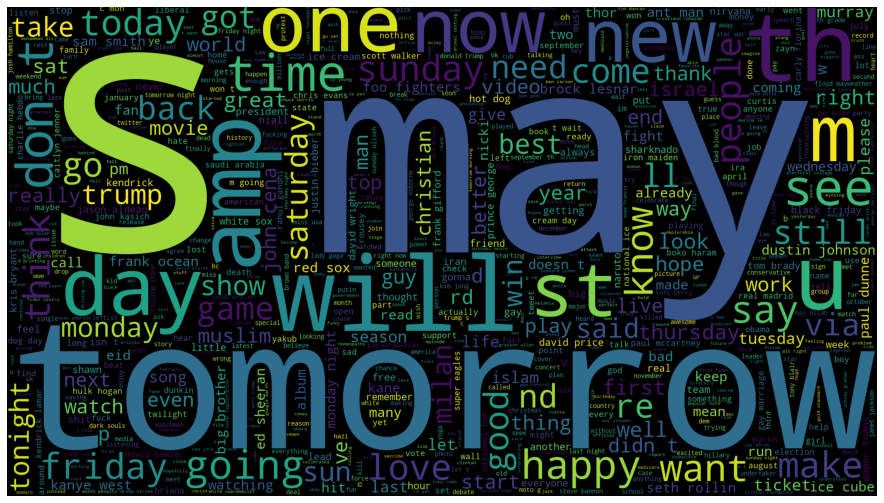
\includegraphics[width = 0.42\textwidth]{wc/text-clean-no-stopwords.png}
	\caption{Word cloud over the cleaned tweets without stopword removal}
	\label{fig:wc-nosw}
\end{figure} 

\begin{figure}[!h]
	\centering
	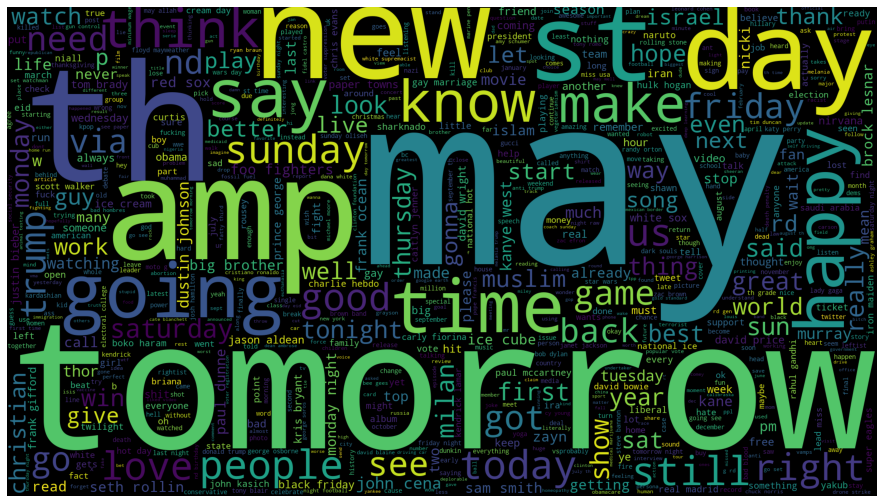
\includegraphics[width = 0.42\textwidth]{wc/all-clean-nltk.png}
	\caption{Word cloud over the cleaned tweets with removal using the \texttt{NLTK} list}
	\label{fig:wc-nltk}
\end{figure} 

\begin{figure}[!h]
	\centering
	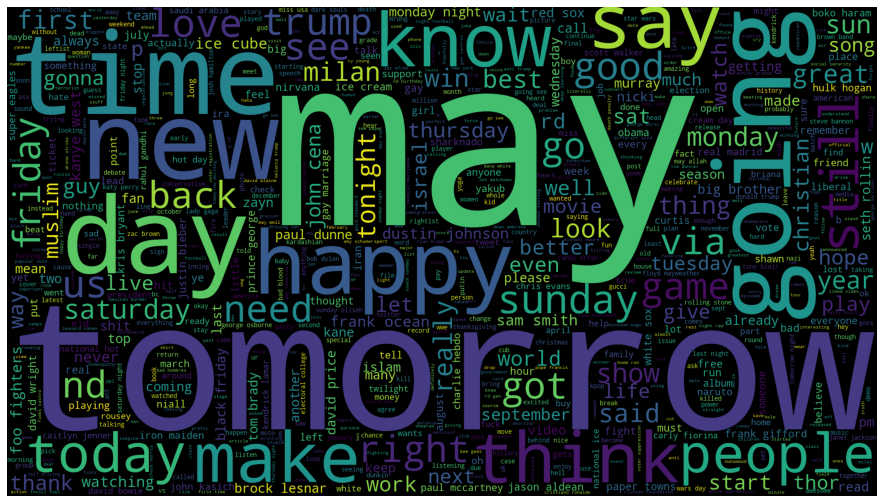
\includegraphics[width = 0.42\textwidth]{wc/all-clean-final.png}
	\caption{Word cloud over the cleaned tweets with removal using the modified \texttt{NLTK} list}
	\label{fig:wc-final}
\end{figure} 

\subsection{Highest cross-validation accuracy per number of maximum features}\label{sec:mfresults}

After generating calssifiers for each of the following values $M_f$, the following boasted the highest scores calculated using Section~\ref{sec:choosing2}.

\begin{table}[!h]
	\begin{center}
		\begin{tabular}{|l|l|}			
			\hline
			Parameter & Value \\
			\hline\hline
			Classifier & Logistic Regression \\
			Fit Intercept & Yes \\
			Maximum Iterations & 500 \\
			Optimizer Algorithm & \texttt{sag} \\
			\hline\hline
			Accuracy &  0.5529\\
			Standard Deviation &  0.04754 \\
			\hline
		\end{tabular}
		\caption{Top classifier for $M_f = 10$}
		\label{tbl:mf10}
	\end{center}
\end{table}

\begin{table}[!h]
	\begin{center}
		\begin{tabular}{|l|l|}			
			\hline
			Parameter & Value \\
			\hline\hline
			Classifier & Logistic Regression \\
			Fit Intercept & Yes \\
			Maximum Iterations & 500 \\
			Optimizer Algorithm & \texttt{sag} \\
			\hline\hline
			Accuracy &  0.5858\\
			Standard Deviation &  0.03109 \\
			\hline
		\end{tabular}
		\caption{Top classifier for $M_f = 100$}
		\label{tbl:mf100}
	\end{center}
\end{table}

\begin{table}[!h]
	\begin{center}
		\begin{tabular}{|l|l|}			
			\hline
			Parameter & Value \\
			\hline\hline
			Classifier & Bernoulli NB \\
			Include Priors & Yes \\
			$\alpha$ Smoothing & 1 \\
			\hline\hline
			Accuracy &  0.6054\\
			Standard Deviation &  0.01067 \\
			\hline
		\end{tabular}
		\caption{Top classifier for $M_f = 1000$}
		\label{tbl:mf1000}
	\end{center}
\end{table}


\begin{table}[!h]
	\begin{center}
		\begin{tabular}{|l|l|}			
			\hline
			Parameter & Value \\
			\hline\hline
			Classifier & Bernoulli NB \\
			Include Priors & Yes \\
			$\alpha$ Smoothing & 1 \\
			\hline\hline
			Accuracy &  0.6321\\
			Standard Deviation &  0.01504 \\
			\hline
		\end{tabular}
		\caption{Top classifier for $M_f = 5000$}
		\label{tbl:mf5000}
	\end{center}
\end{table}

\begin{table}[!h]
	\begin{center}
		\begin{tabular}{|l|l|}			
			\hline
			Parameter & Value \\
			\hline\hline
			Classifier & Bernoulli NB \\
			Include Priors & Yes \\
			$\alpha$ Smoothing & 1 \\
			\hline\hline
			Accuracy &  0.6329\\
			Standard Deviation &   0.01237 \\
			\hline
		\end{tabular}
		\caption{Top classifier for $M_f = 10000$}
		\label{tbl:mf10000}
	\end{center}
\end{table}

Since the model accuracy begins to plateau at $M_f = 10000$,
The final classifer models are constructed using $M_f = 10000$ as an upper bound for features per feature type.

\subsection{The top 3 parameter/classifier configurations}\label{sec:top3}

The following parameter configurations yield the 3 highest scores as defined in Section~\ref{sec:choosing2}

\begin{table}[!h]
	\begin{center}
		\begin{tabular}{|l|l|}			
			\hline
			Parameter & Value \\
			\hline\hline
			Classifier & Bernoulli NB \\
			Include Priors & Yes \\
			$\alpha$ Smoothing & 1 \\
			\hline\hline
			Accuracy &  0.6329\\
			Standard Deviation &   0.01237 \\
			\hline
		\end{tabular}
		\caption{Top classifier (Classifier 1) for $M_f = 10000$}
		\label{tbl:1st10000}
	\end{center}
\end{table}

\begin{table}[!h]
	\begin{center}
		\begin{tabular}{|l|l|}			
			\hline
			Parameter & Value \\
			\hline\hline
			Classifier & Bernoulli NB \\
			Include Priors & No \\
			$\alpha$ Smoothing & 1 \\
			\hline\hline
			Accuracy &  0.6319\\
			Standard Deviation &   0.01210 \\
			\hline
		\end{tabular}
		\caption{2nd best classifier (Classifier 2) for $M_f = 10000$}
		\label{tbl:2nd10000}
	\end{center}
\end{table}

\begin{table}[!h]
	\begin{center}
		\begin{tabular}{|l|l|}			
			\hline
			Parameter & Value \\
			\hline\hline
			Classifier & Multinomial NB \\
			Include Priors & Yes \\
			$\alpha$ Smoothing & 1 \\
			\hline\hline
			Accuracy &  0.6319\\
			Standard Deviation &   0.01210 \\
			\hline
		\end{tabular}
		\caption{3rd best classifier (Classifier 3) for $M_f = 10000$}
		\label{tbl:3rd10000}
	\end{center}
\end{table}

It appears that the top classifiers according to the used scoring value are all Naive Bayes classifiers.

\subsection{Generating evaluation metrics for the final 4 models}

Generated based on Section~\ref{sec:evalmetrics}. 
Per-class metrics are shown in order of postive, neutral, then negative sentiments.

\begin{table}[!h]
	\begin{center}
		\begin{tabular}{|l|l|}			
			\hline
			Parameter & Value \\
			\hline\hline
			Classifier & 0-R \\
			\hline\hline
			Training & Uniform \\
			Testing & Uniform \\
			\hline
			Accuracy & 0.33 \\
			Precisions (+, n, --) 	& 0.00, 0.00, 0.33 \\
			Recalls (+, n, --) 		& 0.00, 0.00, 1.00 \\
			$F_1$ Scores (+, n, --) & 0.00, 0.00, 0.50 \\
			\hline\hline
			Training & Random \\
			Testing & Random \\
			\hline
			Accuracy & 0.58 \\
			Precisions (+, n, --) 	& 0.00, 0.58, 0.00 \\
			Recalls (+, n, --) 		& 0.00, 1.00, 0.00 \\
			$F_1$ Scores (+, n, --) & 0.00, 0.73, 0.00 \\
			\hline\hline
			Training & Random \\
			Testing & Uniform \\
			\hline
			Accuracy & 0.33 \\
			Precisions (+, n, --) 	& 0.00, 0.33, 0.00 \\
			Recalls (+, n, --) 		& 0.00, 1.00, 0.00 \\
			$F_1$ Scores (+, n, --) & 0.00, 0.50, 0.00 \\
			\hline\hline
			Training & Uniform \\
			Testing & Random \\
			\hline
			Accuracy & 0.17 \\
			Precisions (+, n, --) &  0.00, 0.00, 0.17 \\
			Recalls (+, n, --) & 0.00, 0.00, 1.00 \\
			$F_1$ Scores (+, n, --) & 0.00, 0.00, 0.29 \\
			\hline
		\end{tabular}
		\caption{Metrics of Baseline classifier for $M_f = 10000$}
		\label{tbl:metrics-base10000}
	\end{center}
\end{table}

\begin{figure}[!h]
	\centering
	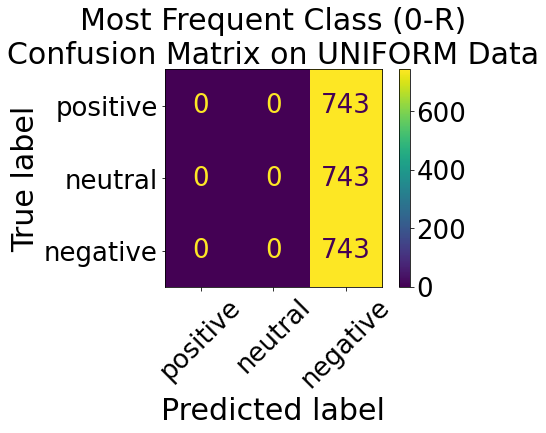
\includegraphics[width = 0.42\textwidth]{cf/MostFrequentClass0R-Uniform-confusion-matrix.png}
	\caption{Baseline classifier's confusion matrix for uniform training and uniform testing data}
	\label{fig:cf-base-uu}
\end{figure} 

\begin{figure}[!h]
	\centering
	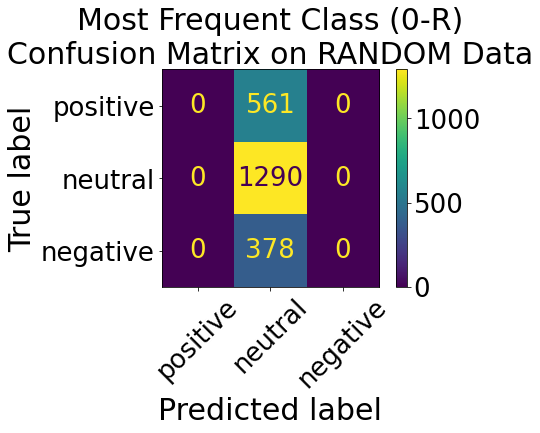
\includegraphics[width = 0.42\textwidth]{cf/MostFrequentClass0R-Random-confusion-matrix.png}
	\caption{Baseline classifier's confusion matrix for random training and random testing data}
	\label{fig:cf-base-rr}
\end{figure} 

\begin{figure}[!h]
	\centering
	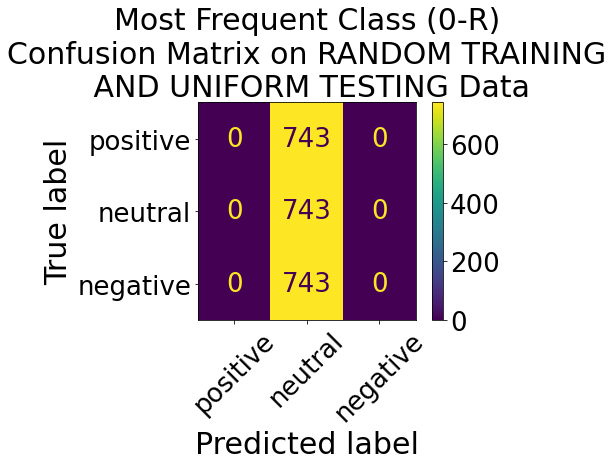
\includegraphics[width = 0.42\textwidth]{cf/MostFrequentClass0R-RandomTrainingandUniformTesting-confusion-matrix.png}
	\caption{Baseline classifier's confusion matrix for random training and uniform testing data}
	\label{fig:cf-base-ru}
\end{figure} 

\begin{figure}[!h]
	\centering
	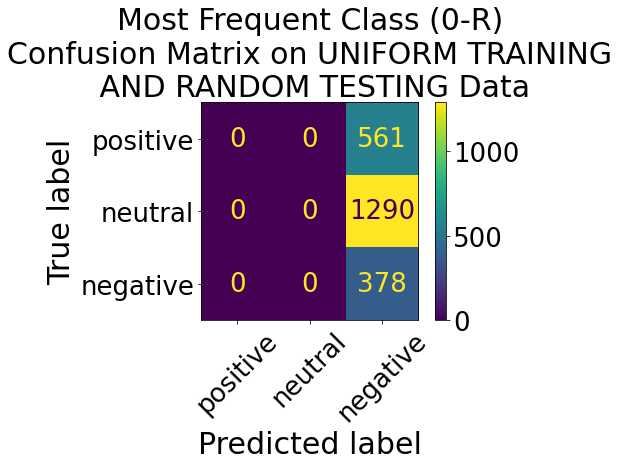
\includegraphics[width = 0.42\textwidth]{cf/MostFrequentClass0R-UniformTrainingandRandomTesting-confusion-matrix.png}
	\caption{Baseline classifier's confusion matrix for uniform training and random testing data}
	\label{fig:cf-base-ur}
\end{figure} 


\begin{table}[!h]
	\begin{center}
		\begin{tabular}{|l|l|}			
			\hline
			Parameter & Value \\
			\hline\hline
			Classifier & Bernoulli NB \\
			Include Priors & Yes \\
			$\alpha$ Smoothing & 1 \\
			\hline\hline
			Training & Uniform \\
			Testing & Uniform \\
			\hline
			Accuracy & 0.62 \\
			Precisions (+, n, --) &  0.65, 0.54, 0.64 \\
			Recalls (+, n, --) & 0.69, 0.43, 0.73 \\
			$F_1$ Scores (+, n, --) & 0.67, 0.48, 0.68 \\
			\hline\hline
			Training & Random \\
			Testing & Random \\
			\hline
			Accuracy & 0.61 \\
			Precisions (+, n, --) &  0.78, 0.60, 0.50 \\
			Recalls (+, n, --) & 0.14, 0.98, 0.74 \\
			$F_1$ Scores (+, n, --) & 0.24, 0.74, 0.01 \\
			\hline\hline
			Training & Random \\
			Testing & Uniform \\
			\hline
			Accuracy & 0.41 \\
			Precisions (+, n, --) &  0.94, 0.36, 1.00 \\
			Recalls (+, n, --) & 0.21, 0.99, 0.02 \\
			$F_1$ Scores (+, n, --) & 0.35, 0.53, 0.04 \\
			\hline\hline
			Training & Uniform \\
			Testing & Random \\
			\hline
			Accuracy & 0.64 \\
			Precisions (+, n, --) &  0.56, 0.87, 0.48 \\
			Recalls (+, n, --) & 0.81, 0.51, 0.84 \\
			$F_1$ Scores (+, n, --) & 0.66, 0.64, 0.61 \\
			\hline
		\end{tabular}
		\caption{Metrics of Classifier 1 for $M_f = 10000$}
		\label{tbl:metrics-1st10000}
	\end{center}
\end{table}

\begin{figure}[!h]
	\centering
	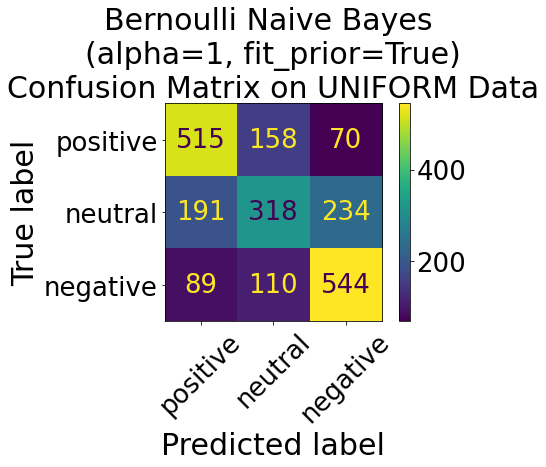
\includegraphics[width = 0.42\textwidth]{cf/BernoulliNaiveBayesalpha1fit_priorTrue-Uniform-confusion-matrix.png}
	\caption{Classifier 1's confusion matrix for uniform training and uniform testing data}
	\label{fig:cf-1st-uu}
\end{figure} 

\begin{figure}[!h]
	\centering
	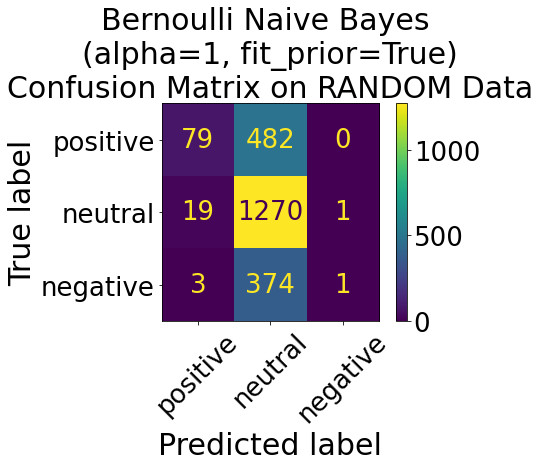
\includegraphics[width = 0.42\textwidth]{cf/BernoulliNaiveBayesalpha1fit_priorTrue-Random-confusion-matrix.png}
	\caption{Classifier 1's confusion matrix for random training and random testing data}
	\label{fig:cf-1st-rr}
\end{figure} 

\begin{figure}[!h]
	\centering
	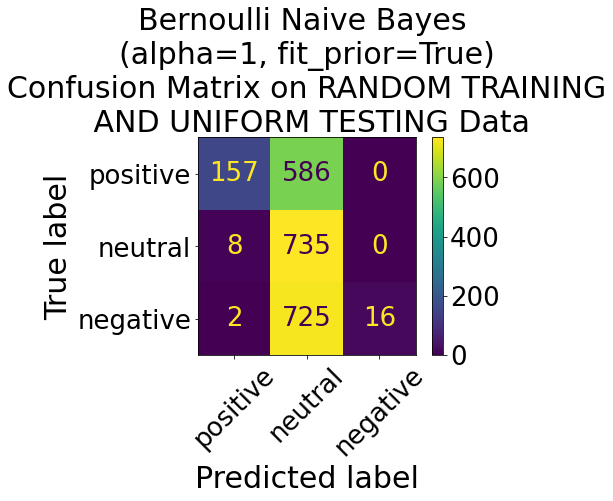
\includegraphics[width = 0.42\textwidth]{cf/BernoulliNaiveBayesalpha1fit_priorTrue-RandomTrainingandUniformTesting-confusion-matrix.png}
	\caption{Classifier 1's confusion matrix for random training and uniform testing data}
	\label{fig:cf-1st-ru}
\end{figure} 

\begin{figure}[!h]
	\centering
	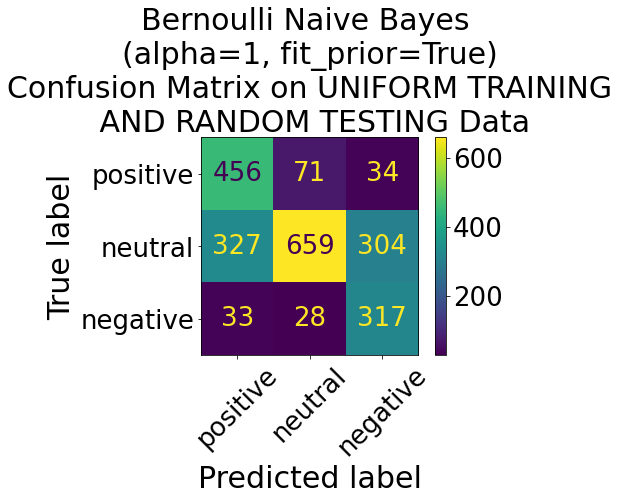
\includegraphics[width = 0.42\textwidth]{cf/BernoulliNaiveBayesalpha1fit_priorTrue-UniformTrainingandRandomTesting-confusion-matrix.png}
	\caption{Classifier 1's confusion matrix for uniform training and random testing data}
	\label{fig:cf-1st-ur}
\end{figure} 


\begin{table}[!h]
	\begin{center}
		\begin{tabular}{|l|l|}			
			\hline
			Parameter & Value \\
			\hline\hline
			Classifier & Bernoulli NB \\
			Include Priors & No \\
			$\alpha$ Smoothing & 1 \\
			\hline\hline
			Training & Uniform \\
			Testing & Uniform \\
			\hline
			Accuracy & 0.62 \\
			Precisions (+, n, --) &  0.65, 0.54, 0.64 \\
			Recalls (+, n, --) & 0.69, 0.43, 0.73 \\
			$F_1$ Scores (+, n, --) & 0.67, 0.48, 0.68 \\
			\hline\hline
			Training & Random \\
			Testing & Random \\
			\hline
			Accuracy & 0.61 \\
			Precisions (+, n, --) &  0.74, 0.60, 0.75 \\
			Recalls (+, n, --) & 0.17, 0.98, 0.01 \\
			$F_1$ Scores (+, n, --) & 0.27, 0.74, 0.02 \\
			\hline\hline
			Training & Random \\
			Testing & Uniform \\
			\hline
			Accuracy & 0.42 \\
			Precisions (+, n, --) &  0.91, 0.36, 0.96 \\
			Recalls (+, n, --) & 0.25, 0.98, 0.04 \\
			$F_1$ Scores (+, n, --) & 0.39, 0.53, 0.07 \\
			\hline\hline
			Training & Uniform \\
			Testing & Random \\
			\hline
			Accuracy & 0.64 \\
			Precisions (+, n, --) &  0.56, 0.87, 0.48 \\
			Recalls (+, n, --) & 0.81, 0.51, 0.84 \\
			$F_1$ Scores (+, n, --) & 0.66, 0.64, 0.61 \\
			\hline
		\end{tabular}
		\caption{Metrics of Classifer 2 for $M_f = 10000$}
		\label{tbl:metrics-2nd10000}
	\end{center}
\end{table}

\begin{figure}[!h]
	\centering
	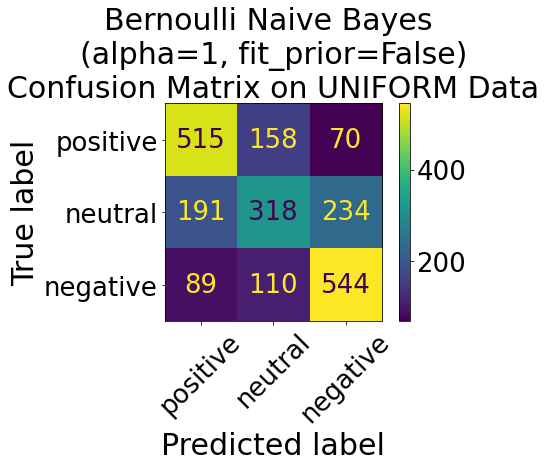
\includegraphics[width = 0.42\textwidth]{cf/BernoulliNaiveBayesalpha1fit_priorFalse-Uniform-confusion-matrix.png}
	\caption{Classifier 2's confusion matrix for uniform training and uniform testing data}
	\label{fig:cf-2nd-uu}
\end{figure} 

\begin{figure}[!h]
	\centering
	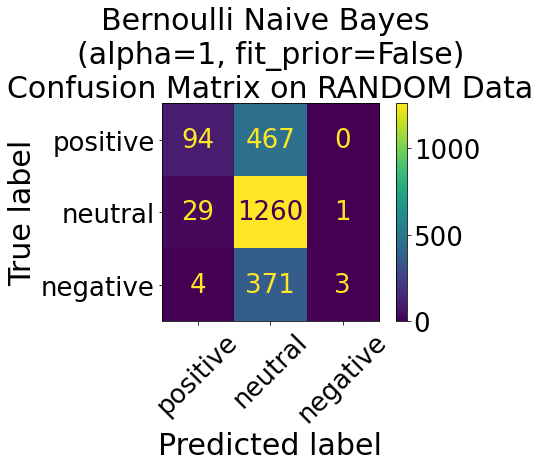
\includegraphics[width = 0.42\textwidth]{cf/BernoulliNaiveBayesalpha1fit_priorFalse-Random-confusion-matrix.png}
	\caption{Classifier 2's confusion matrix for random training and random testing data}
	\label{fig:cf-2nd-rr}
\end{figure} 

\begin{figure}[!h]
	\centering
	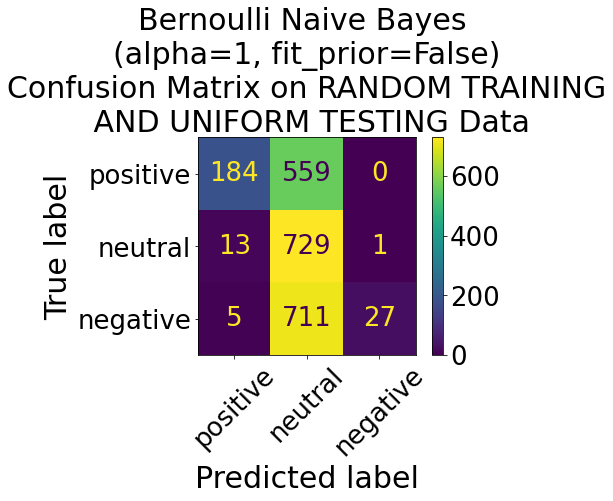
\includegraphics[width = 0.42\textwidth]{cf/BernoulliNaiveBayesalpha1fit_priorFalse-RandomTrainingandUniformTesting-confusion-matrix.png}
	\caption{Classifier 2's confusion matrix for random training and uniform testing data}
	\label{fig:cf-2nd-ru}
\end{figure} 

\begin{figure}[!h]
	\centering
	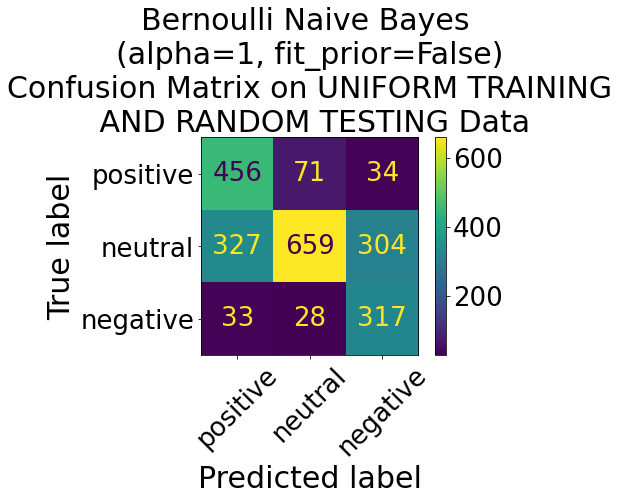
\includegraphics[width = 0.42\textwidth]{cf/BernoulliNaiveBayesalpha1fit_priorFalse-UniformTrainingandRandomTesting-confusion-matrix.png}
	\caption{Classifier 2's confusion matrix for uniform training and random testing data}
	\label{fig:cf-2nd-ur}
\end{figure} 

\begin{table}[!h]
	\begin{center}
		\begin{tabular}{|l|l|}			
			\hline
			Parameter & Value \\
			\hline\hline
			Classifier & Multinomial NB \\
			Include Priors & Yes \\
			$\alpha$ Smoothing & 1 \\
			\hline\hline
			Training & Uniform \\
			Testing & Uniform \\
			\hline
			Accuracy & 0.62 \\
			Precisions (+, n, --) &  0.66, 0.57, 0.62 \\
			Recalls (+, n, --) & 0.66, 0.42, 0.78 \\
			$F_1$ Scores (+, n, --) & 0.66, 0.48, 0.69 \\
			\hline\hline
			Training & Random \\
			Testing & Random \\
			\hline
			Accuracy & 0.61 \\
			Precisions (+, n, --) &  0.76, 0.60, 0.60 \\
			Recalls (+, n, --) & 0.19, 0.97, 0.01 \\
			$F_1$ Scores (+, n, --) & 0.30, 0.75, 0.02 \\
			\hline\hline
			Training & Random \\
			Testing & Uniform \\
			\hline
			Accuracy & 0.42 \\
			Precisions (+, n, --) &  0.92, 0.36, 1.00 \\
			Recalls (+, n, --) & 0.26, 0.98, 0.02 \\
			$F_1$ Scores (+, n, --) & 0.41, 0.53, 0.04 \\
			\hline\hline
			Training & Uniform \\
			Testing & Random \\
			\hline
			Accuracy & 0.62 \\
			Precisions (+, n, --) &  0.57, 0.87, 0.44 \\
			Recalls (+, n, --) & 0.78, 0.48, 0.87 \\
			$F_1$ Scores (+, n, --) & 0.66, 0.62, 0.59 \\
			\hline
		\end{tabular}
		\caption{Metrics of Classifer 3 for $M_f = 10000$}
		\label{tbl:metrics-3rd10000}
	\end{center}
\end{table}

\begin{figure}[!h]
	\centering
	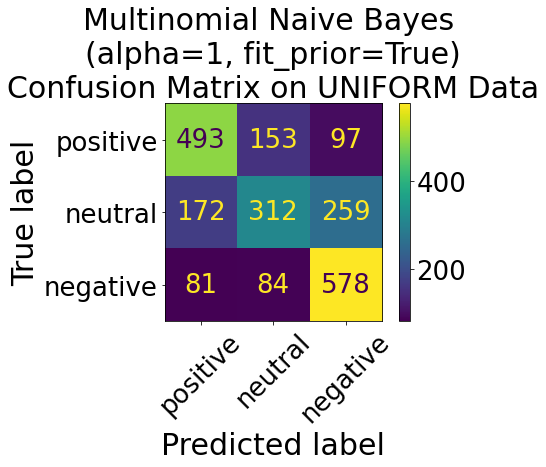
\includegraphics[width = 0.42\textwidth]{cf/MultinomialNaiveBayesalpha1fit_priorTrue-Uniform-confusion-matrix.png}
	\caption{Classifier 3's confusion matrix for uniform training and uniform testing data}
	\label{fig:cf-3rd-uu}
\end{figure} 

\begin{figure}[!h]
	\centering
	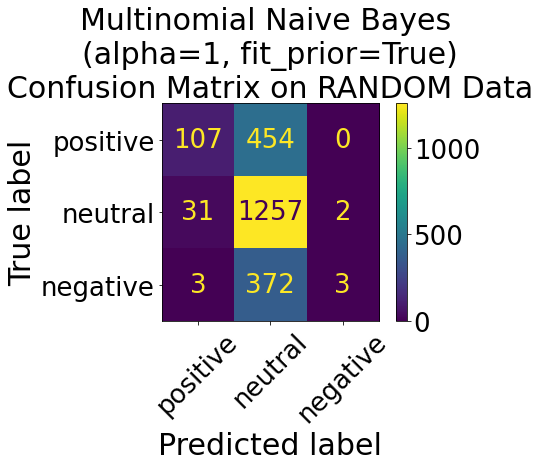
\includegraphics[width = 0.42\textwidth]{cf/MultinomialNaiveBayesalpha1fit_priorTrue-Random-confusion-matrix.png}
	\caption{Classifier 3's confusion matrix for random training and random testing data}
	\label{fig:cf-3rd-rr}
\end{figure} 

\begin{figure}[!h]
	\centering
	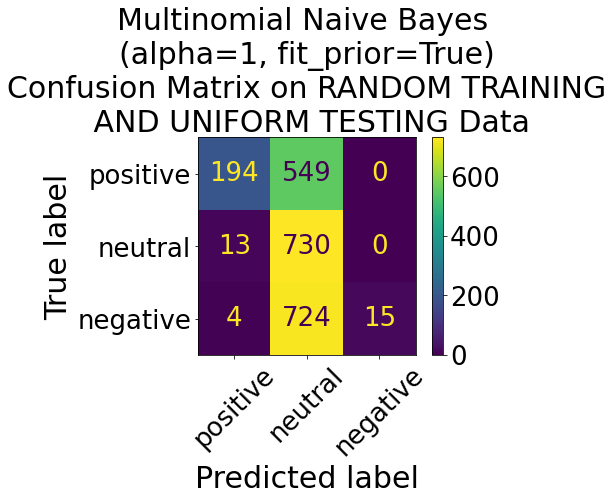
\includegraphics[width = 0.42\textwidth]{cf/MultinomialNaiveBayesalpha1fit_priorTrue-RandomTrainingandUniformTesting-confusion-matrix.png}
	\caption{Classifier 3's confusion matrix for random training and uniform testing data}
	\label{fig:cf-3rd-ru}
\end{figure} 

\begin{figure}[!h]
	\centering
	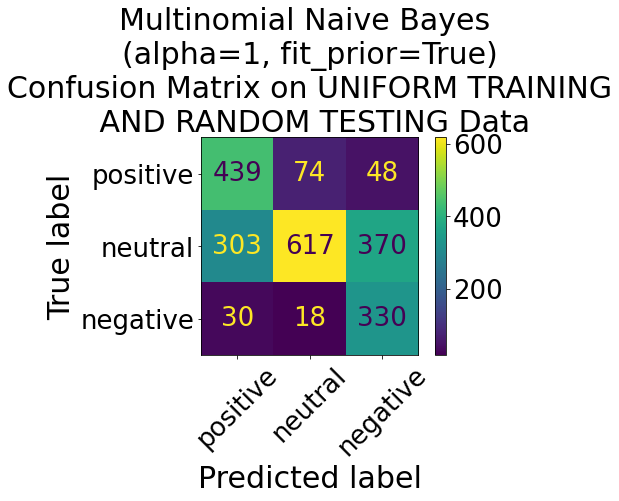
\includegraphics[width = 0.42\textwidth]{cf/MultinomialNaiveBayesalpha1fit_priorTrue-UniformTrainingandRandomTesting-confusion-matrix.png}
	\caption{Classifier 3's confusion matrix for uniform training and random testing data}
	\label{fig:cf-3rd-ur}
\end{figure} 



\section{Analysis}
% Discussion / Critical Analysis: Contextualise the systems' behaviour, based on the understanding of the
% subject materials (This is the most important part of the task in this assignment).

% Contextualise implies that we are more interested in seeing evidence of you have thought about the task
% and determining reasons for the relative performance of different methods, rather than the raw scores of
% the different methods you selected. This is not to say that you should ignore the relative performance of
% different runs over the data, but rather that you should think beyond simple numbers to the reasons that
% underlie them.

\subsection{How the stopword removal modifies the data}
The cleaning technique used highlights a large number of unformed word parts, such as ``\emph{s}'' or ``\emph{u}'', as shown in Figure~\ref{fig:wc-nosw}.
The initial stopword list misses some highly repeated terms with no meaning (e.g. ``\emph{th}'') as is displayed in Figure~\ref{fig:wc-nltk}. 
These terms need to be removed manually, to yield a final word cloud shown in Figure~\ref{fig:wc-final}.
Although words like ``\emph{tomorrow}'' appear frequently, they may be parts of sentiment indicative word 2-grams (e.g. ``\emph{happy tomorrow}''), and are therefore not removed.

\subsection{How the maximum number of features per feature type $M_f$ modifies the models}
The results shown in Section~\ref{sec:mfresults} highlight an interesting pattern in the classifiers.
For lower max feature values $M_f$, the highest performing model is the logistic regression,
whereas past $M_f = 1000$, the best model is the Bernoulli Naive Bayes. 
This suggests that logistic regressions are better for smaller dimensions of features.
This is likely due to the logistic regressions reliance on optimization to find the best model.
Since optimization is perfomed to find local minima in errors in the model, 
a smaller feature space results in fewer local minima, 
and therefore a higher likelihood in the local minimum being the overall minimum of errors.
The results also highlight the Bernoulli Naive Bayes model, as it yields the highest 80\% accuracy for larger feature spaces.
Most of the classifiers considered rely on solving an optimization problem to determine a support vector, or a set of weights.
The Naive Bayes models do rely on optimization, and are therefore more reliable in complex feature spaces.

\subsection{The best classifier/parameter configurations}

The three best model configurations for a large feature space are Naive Bayes estimators, as shown in Section~\ref{sec:top3}.
The highest scoring model is the Bernoulli Naive Bayes, with $\alpha = 1$ laplace smoothing and sentiment label priors included.


Both multinomial and bernoulli naive bayes classifiers are very similar in function, one relies on multiple possible events, whereas the other relies on binary events.
With this data and feature set, the bernoulli naive bayes classifier tends to be more applicable, since most features either appear or don't appear within a tweet (appear in binary events).
This is reflected in the best possible model, while the multinomial model is still high accuracy relative to non-naive bayes methods (Table~\ref{tbl:3rd10000}).


The naive bayes classifiers tend to yield higher accuracies than the other considered classifiers, since they scale easily with the size of the feature space.
Other models rely on optimization, which increases in complexity with the feature space.
As more features are added, there will be a higher number of possible minima and maxima to consider when optimizing, decreasing the chances of the true best configuration being discovered.
I would need to either start with an initial state that is known to be closest to the most accurate, or to train the models on a large number of iterations.
Both of these options are not realistic with limited time, and with a large feature space as I am using.

\subsection{Of the final 4 models, which are most sentiment distribution agnostic}



\section{Conclusions}
% Conclusion: Demonstrate your identified knowledge about the problem.

\bibliographystyle{acl}
\bibliography{citations}

\end{document}
